% Options for packages loaded elsewhere
\PassOptionsToPackage{unicode}{hyperref}
\PassOptionsToPackage{hyphens}{url}
%
\documentclass[
  twocolumn]{article}
\title{Bayesian Estimation of parameters for Survival models using the
Cox Proportional model}
\author{Daniela Pico Julian Usuga Deivid Zhang}
\date{2022-06-19}

\usepackage{amsmath,amssymb}
\usepackage{lmodern}
\usepackage{iftex}
\ifPDFTeX
  \usepackage[T1]{fontenc}
  \usepackage[utf8]{inputenc}
  \usepackage{textcomp} % provide euro and other symbols
\else % if luatex or xetex
  \usepackage{unicode-math}
  \defaultfontfeatures{Scale=MatchLowercase}
  \defaultfontfeatures[\rmfamily]{Ligatures=TeX,Scale=1}
\fi
% Use upquote if available, for straight quotes in verbatim environments
\IfFileExists{upquote.sty}{\usepackage{upquote}}{}
\IfFileExists{microtype.sty}{% use microtype if available
  \usepackage[]{microtype}
  \UseMicrotypeSet[protrusion]{basicmath} % disable protrusion for tt fonts
}{}
\makeatletter
\@ifundefined{KOMAClassName}{% if non-KOMA class
  \IfFileExists{parskip.sty}{%
    \usepackage{parskip}
  }{% else
    \setlength{\parindent}{0pt}
    \setlength{\parskip}{6pt plus 2pt minus 1pt}}
}{% if KOMA class
  \KOMAoptions{parskip=half}}
\makeatother
\usepackage{xcolor}
\IfFileExists{xurl.sty}{\usepackage{xurl}}{} % add URL line breaks if available
\IfFileExists{bookmark.sty}{\usepackage{bookmark}}{\usepackage{hyperref}}
\hypersetup{
  pdftitle={Bayesian Estimation of parameters for Survival models using the Cox Proportional model},
  pdfauthor={Daniela Pico Julian Usuga Deivid Zhang},
  hidelinks,
  pdfcreator={LaTeX via pandoc}}
\urlstyle{same} % disable monospaced font for URLs
\usepackage[margin=1in]{geometry}
\usepackage{graphicx}
\makeatletter
\def\maxwidth{\ifdim\Gin@nat@width>\linewidth\linewidth\else\Gin@nat@width\fi}
\def\maxheight{\ifdim\Gin@nat@height>\textheight\textheight\else\Gin@nat@height\fi}
\makeatother
% Scale images if necessary, so that they will not overflow the page
% margins by default, and it is still possible to overwrite the defaults
% using explicit options in \includegraphics[width, height, ...]{}
\setkeys{Gin}{width=\maxwidth,height=\maxheight,keepaspectratio}
% Set default figure placement to htbp
\makeatletter
\def\fps@figure{htbp}
\makeatother
\setlength{\emergencystretch}{3em} % prevent overfull lines
\providecommand{\tightlist}{%
  \setlength{\itemsep}{0pt}\setlength{\parskip}{0pt}}
\setcounter{secnumdepth}{-\maxdimen} % remove section numbering
\ifLuaTeX
  \usepackage{selnolig}  % disable illegal ligatures
\fi

\begin{document}
\maketitle

\hypertarget{abstract}{%
\section{Abstract}\label{abstract}}

The main objective of the study was to predict the mortality of people
in African countries. Using data from the DHS and functions from the
\emph{mortDHS} package, functions were created for any given country
within the set of DHS surveys, a useful model is generated to make
predictions of survival and evaluate the effects associated with it, a
measurement that cannot be made from non-parametric models such as
Kaplan-Meier (as initially proposed in the study). Specifically, a
discrimination is obtained between the differences in the survival of
each person depending on their sex and country, these predictions are
made from a Bayesian approach using the \emph{Rstanarm} package, which
uses the Stan software to make its estimates.

\hypertarget{introduction}{%
\section{Introduction}\label{introduction}}

\hypertarget{the-problem}{%
\subsection{The problem}\label{the-problem}}

In our study we were interested in estimating the mortality on African
countries. These countries sometimes lack of a good and reliable
registry of deaths and without these estimating mortality rates can be
difficult, these rates have prime importance on epidemiological or
socio-economic studies.

In our study we used the survey data provided by DHS, these contain a
large number of variables, people were asked about the survival status
of their siblings so we only include sibling data on our study, we
assess siblings survival, expecting to derivate from these the mortality
of the population.

\hypertarget{study-population}{%
\subsection{Study Population}\label{study-population}}

Many countries don't have good registries management on government
institutions and thus they don't have a good record of important events
such as population deaths, the Demographic and Health Surveys (DHS)
facilitates multiple datasets containing data collected from
questionnaires performed in households from a large list of countries.

In our study we will consider the Individual Women's data, which consist
of questionnaires performed to women. They were asked about wherever
they had siblings, their survival status, age and death date (in case
they have died).

\hypertarget{data-source}{%
\subsection{Data source}\label{data-source}}

The primary data source was the Demographic and Health Surveys (DHS)
Individual Recode (IR) where each row consist of a woman and their
responses on multiple questions. There were multiple columns but we
selected the ones related to siblings and their survival status, these
where:

\begin{itemize}
\tightlist
\item
  Sibling sex (male or female)
\item
  Sibling date of birth
\item
  Sibling survival status (0 = dead, 1 = alive)
\item
  Sibling date of death
\end{itemize}

\hypertarget{basic-concepts}{%
\section{Basic concepts}\label{basic-concepts}}

\hypertarget{survival-analysis}{%
\subsection{Survival analysis}\label{survival-analysis}}

Survival analysis is a collection of statistical methods for study the
time that elapses until an event occurs {[}1{]}. The name survival is
due to the fact that the applications of this method are mainly study
the times of death, some fields of the application of survival analysis
They include: medicine, epidemiology, economics, among others. An
advantage of models based on survival analysis is that they allow work
with censored data, censoring occurs when you have some information on
the survival time of a patient but the exact time to failure is not
known.

There are three functions of interest for survival analysis, the
survival function denoted \(S(t)\), the hazard function denoted
\(h(t)\), and the hazard function accumulated denoted by \(H(t)\), these
will be the amounts of interest for our study. According to the
literature {[}2{]}, functions are defined as follows:

Let \(T\) be a random variable denoting the survival time of a unit or
person. The survival function, which is denoted \(S(t)\) gives the
probability that a unit or person will survives beyond some specific
time t. i.e,

\[S(t)= P(T>t)\]

The survival function \(S(t)\) is fundamental in AS since for different
values of \(t\) provide crucial information of survival data In some
situations it may be more interest to quantify the risk of failure at a
given instant than to estimate survival; a function of interest in
survival analysis that allows do this is the danger function

The hazard function usually denoted as \(h(t)\) or \(\lambda(t)\) is
given by:

\[ h(t)=\lim_{\Delta t \to 0}\frac{P(t\leq T+\Delta t|T\geq t)}{\Delta t}\]
The numerator represents the conditional probability of the event
occurring in an infinitesimal interval \([t,t+\Delta t]\) (as
\(\Delta t\to 0\)) given that the unit has survived to \(t\) \((T>t)\).
survived until t (T\textgreater t).

The cumulative hazard is defined as:

\[H(t)=\int_{0}^{t}h(s)ds\]

Where \(h(s)\) is the hazard function. exist a one to-one relationship
between the hazard function, the cumulative hazard and the probability
of survival, as follows

\[S(t)=exp(-H(t))=exp(-\int_{0}^{t}h(s)ds)\]

\hypertarget{censorship}{%
\subsection{Censorship}\label{censorship}}

An observation in a random variable \(T\) is said to be right-censored
if all that is known about of \(T\) is that it is greater than some
value c. In AS, \(T\) refers at the time of occurrence of some
particular event and a case is considered right-censored if it stops
observing before for the event to occur{[}3{]}. In our work, only the
right caesura is presented, since at the time of conducting the survey
there were people who had not yet experienced the event of interest
(death).

Survival probability can be estimated non-parametrically over temporal
observations (censored and uncensored) using the Kaplan-Meyer method.
other two Common approaches to modeling survival data consist of
modeling the instantaneous rate of the event as a function of time. This
includes the class of models known as proportional hazards regression
models and non-proportional hazards regression models; the second is to
model the time of the event itself. This includes the class of models
known as accelerated time to failure (AFT) models.

\hypertarget{bayesian-approach-and-why-bayesian}{%
\subsection{Bayesian approach and why
Bayesian}\label{bayesian-approach-and-why-bayesian}}

The main reason to go Bayesian in our study was to be able to make
inference, in particular, to make easy to interpretative conclusions on
our parameters and their significance, without the assumptions of
frecuentists approaches.

\hypertarget{models}{%
\section{Models}\label{models}}

Under this modeling framework, it is proposed to implement a of Bayesian
Cox proportional hazard to later make a comparison versus the
frequentest approach and the kaplan Meier curve.

\hypertarget{kaplanmeier-estimator}{%
\subsection{Kaplan--Meier estimator}\label{kaplanmeier-estimator}}

The Kaplan-Meier estimator, also known as the limit product estimator,
is a nonparametric method for estimating the survival function. survival
function by maximizing the sample likelihood function. Suppose one has k
different failure times \(t_1<t_2<...<t_k\), in each time
\(t_j(j=1,2,...k)\) there are \(n_j\) subjects that are under
observation and at risk of an event of interest.

The K-M estimator is defined as
\[\hat S_{KM}(t)=\prod_{j:t_j\leq t}^{}[1-\frac{d_j}{n_j}]\hspace{2.5mm}\]\[para\hspace{2.5mm}t_1\leq t\leq t_k\hspace{2.5mm}y\hspace{2.5mm}d_j=\#faults\]

\hypertarget{cox-proportional-hazards-model}{%
\subsection{Cox proportional hazards
model}\label{cox-proportional-hazards-model}}

Under a hazard scale formulation, we model the hazard of the event for
individual \(i\) at time \(t\) using the following model:

\[h(t|X_i)=h_0(t)exp(X_i\beta)\]

Where \(h_0\) is called the hazard base, that is, \(h_0(t)\) is the risk
when all \(X_i\) variables are 0. \(h_0(t)\) characterizes the way in
which hazard changes as a function of survival time, while the second
term characterizes the way the hazard changes as function of the
covariates at the same time guarantees that this is positive, it is also
called the linear predictor.

The formulation of the Cox model in terms of the hazard and the survival
function are given by: From (2) we note that \[S(t;x)=exp(-H(t;x))\]
Where \(H(t;\vec{x})\) is the cumulative hazard for a subject with
covariates \(\vec{x}=(x_1,x_2,..x_k)\) Assuming survival time is
continuous

\[H(t;\vec{x})=\int_{0}^{t} h(s;\vec{x})ds=\int_{0}^{t} h_0(s)exp(\beta^T\vec{x})ds\]
\[=exp(\beta^T\vec{x})\int_{0}^{t} h_0(s)ds=
exp(\beta^T\vec{x})H_0(T)\]

Cox model in terms of cumulative hazard. In this expression \(H_0(t)\)
is the cumulative baseline hazard. This relationship can be thought of
as a baseline cumulative risk measure which is modified according to the
function

From the above relationship, the Cox model can be formulated in terms of
survival:

\[S(t;\vec{x})=exp(-H(t;\vec{x}))=exp(e^{\beta^T\vec{x}})H_0(t)=\]
\[[exp(-H_0(t)]^{e^{\beta^T\vec{x}}}=[S_0(t)]^{e^{\beta^T\vec{x}}}\]

Cox model in terms of survival. In this expression \(S_0(t)\) is the
survival baseline.

\hypertarget{estimation}{%
\section{Estimation}\label{estimation}}

As we previously seen, the cox proportional hazard model has two parts,
one is the baseline hazard and the second one is the linear model, for
the linear model we only choose to estimate each of the \(\beta\) using
normal prios, but for the hazard baseline

\hypertarget{linear-model}{%
\subsection{Linear Model}\label{linear-model}}

From the Cox Proportional-Hazards Model we can extract the following
expression, which we call the linear model.

\[
\mathrm{exp}(\beta \cdot X_i)
\]

Where \(\beta = (\beta_0, \beta_1, ... , \beta_n)\) is the vector of
coefficients and \(X_i = (1, x_1, ..., x_n)\) is the vector of
covariables.

On our study the will have vector
\(X_i= (1,\text{I}_{\text{sex = female}}, \text{I}_{\text{country = Rwanda}}, \text{I}_{\text{country = Senegal}})\),
that is because we have two variables and both of them are factors, the
indicator for the male sex and the country Malawi are the reference
absorbed by the intercept \(\beta_0\).

For this particular model we set our priors as such:

\[
\beta_0 \sim N(0, 20)
\]

\[
\beta_{i} \sim N(0,2.5) \ \ \ \text{with   i = 1, 2, 3}
\]

\hypertarget{baseline-hazard}{%
\subsection{Baseline Hazard}\label{baseline-hazard}}

In our study we used an M-Spline model to approximate the hazard
baseline function \(h_0\), this approximation consists of \(\gamma_l\)
coefficients multiplied by each component of the spline, function
calculated inside by the package \textbf{splines2}.

So the hazard of dying for the individual \(i\) at time \(t\) is given
by:\[
h_i(t) = \mathrm{exp}(\beta \cdot X_i)\ast\sum_{l = 1}^{L}\gamma_l \text{M}_l(t \ | \ k, \delta) 
\]Where \(k = \{k_1, ... ,k_J\}\) is a set of knots given by the user,
we observed that a decent number of knots is around 6 (including the 2
boundary knots, \(k_1\) located at the earliest entry time and \(k_J\),
located at the lastest event), this number of knots prevents that our
model is too overfitting, We will leave the default degree of the
splines \(\delta\) at \(3\).

The package \textbf{rstanarm} handles the calculation and sets a
Dirichlet prior with concentration parameter of 1, ensuring an
non-informative prior.

\hypertarget{model-selection}{%
\subsection{Model Selection}\label{model-selection}}

To evaluate the performance of the predictions of each model we use a
cross-validation technique. Through the loo() function that is included
in the \emph{rstanarm} package. The way this package divides the data in
the cross validation is leaving a single observation out, the unit that
is systematically omitted determines the predictive task in which the
cross-validation evaluates the performance of the model, the
computational method implemented is Pareto-smoothed importance sampling.

the Pareto- \(\hat{k}\) diagnostic estimates how far an individual
leave-one-out distribution is from the full distribution. If leaving out
an observation changes the posterior too much then importance sampling
is not able to give reliable estimate. If \(\hat{k}<0.5\), then the
corresponding component of elpd\_loo is estimated with high accuracy. If
\(0.5< \hat{k}<0.7\) the accuracy is lower, but still OK. if
\(\hat{k}>0.7,\) then importance sampling is not able to provide useful
estimate for that component/observation.

The p\_loo is called the effective number of parameters and can be
calculated as the difference between the pd\_loo and the log posterior
predictive density without cross-validation. In well behaving cases
p\_loo\(<N\) and p\_loo \(<p\), where p is the total number of
parameters in the model. p\_loo \(>N\) or p\_loo \(>p\) indicates that
the model has very weak predictive capability.

Evaluating the predictive capacity of each model, it was obtained that
the best performance is given by the model that specifies the hazard
baseline as a spline, so our work will be developed based on this model,
these results are attached in the annex. newpage \newpage

\hypertarget{results}{%
\section{Results}\label{results}}

\hypertarget{estimate}{%
\subsection{Estimate}\label{estimate}}

\begin{table}[h!]
\begin{center}
\begin{tabular}{|l|l|l|l|l|l|}
\hline
          & mean   & sd    & 10\%   & 50\%   \\ \hline
Intercept & -0.891 & 0.161 & -1.087 & -0.907 \\ \hline
sex2      & -0.235 & 0.069 & -0.327 & -0.234 \\ \hline
countryrw & 0.326  & 0.080 & 0.224  & 0.326  \\ \hline
countryse & -0.326  & 0.095 & -0.446  & -0.327  \\ \hline
\end{tabular}
\caption{parameter estimation bayesian approach}
\end{center}
\end{table}

\begin{table}[h!]
\begin{center}
\begin{tabular}{|l|l|l|l|l|l|}
\hline
          & coef     & exp(coef) & se(coef) \\ \hline
sex2      & -0.23247 & 0.79257   & 0.06862\\ \hline
countryrw & 0.32528  & 1.38441   & 0.08013 \\ \hline
countryse & -0.33077 & 0.71837   & 0.09340 \\ \hline
\end{tabular}
\caption{parameter estimation frequentist approach}
\end{center}
\end{table}

\hypertarget{annexes}{%
\section{Annexes}\label{annexes}}

\begin{table}[h!]
\begin{center}
\begin{tabular}{|l|l|l|l|l|l|}
\hline
          & mcse   & Rhat    & n\_eff \\ \hline
Intercept & 0.004  & 1.002   & 1432  \\ \hline
sex2      & 0.001  & 1.000   & 3866 \\ \hline
countryrw & 0.001  & 1.001   & 3419 \\ \hline
countryse & 0.002  & 1.001   & 3404 \\ \hline
\end{tabular}
\caption{MCMC diagnostics}
\end{center}
\end{table}

\begin{table}[h!]
\begin{center}
\begin{tabular}{|lll|}
\hline
\multicolumn{1}{|l|}{}          & \multicolumn{1}{l|}{Estimate} & SE    \\ \hline
\multicolumn{1}{|l|}{elpd\_loo} & \multicolumn{1}{l|}{-7089.7}  & 197.5 \\ \hline
\multicolumn{1}{|l|}{p\_loo}    & \multicolumn{1}{l|}{8.3}      & 0.3   \\ \hline
\multicolumn{1}{|l|}{looic}     & \multicolumn{1}{l|}{14179.5}  & 395.1 \\ \hline
\multicolumn{3}{|l|}{Monte Carlo SE of elpd\_loo is 0.0.}               \\ \hline
\multicolumn{3}{|l|}{All Pareto k estimates are good (k \textless 0.5)} \\ \hline
\end{tabular}
\caption{loo splines}
\end{center}
\end{table}

\begin{table}[h!]
\begin{center}
\begin{tabular}{|lll|}
\hline
\multicolumn{1}{|l|}{}          & \multicolumn{1}{l|}{Estimate} & SE    \\ \hline
\multicolumn{1}{|l|}{elpd\_loo} & \multicolumn{1}{l|}{-7429.6}  & 205.2 \\ \hline
\multicolumn{1}{|l|}{p\_loo}    & \multicolumn{1}{l|}{4.2}      & 0.1   \\ \hline
\multicolumn{1}{|l|}{looic}     & \multicolumn{1}{l|}{14859.1}  & 410.4 \\ \hline
\multicolumn{3}{|l|}{Monte Carlo SE of elpd\_loo is 0.0.}               \\ \hline
\multicolumn{3}{|l|}{All Pareto k estimates are good (k \textless 0.5)} \\ \hline
\end{tabular}
\caption{loo exponential}
\end{center}
\end{table}

\begin{table}[h!]
\begin{center}
\begin{tabular}{|lll|}
\hline
\multicolumn{1}{|l|}{}          & \multicolumn{1}{l|}{Estimate} & SE    \\ \hline
\multicolumn{1}{|l|}{elpd\_loo} & \multicolumn{1}{l|}{-7187.3}  & 199.7 \\ \hline
\multicolumn{1}{|l|}{p\_loo}    & \multicolumn{1}{l|}{4.8}      & 0.1  \\ \hline
\multicolumn{1}{|l|}{looic}     & \multicolumn{1}{l|}{14374.7}  & 399.4 \\ \hline
\multicolumn{3}{|l|}{Monte Carlo SE of elpd\_loo is 0.0.}               \\ \hline
\multicolumn{3}{|l|}{All Pareto k estimates are good (k \textless 0.5)} \\ \hline
\end{tabular}
\caption{loo Weibull}
\end{center}
\end{table}

\begin{table}[h!]
\begin{center}
\begin{tabular}{|l|l|l|}
\hline
             & elpd\_diff & se\_diff \\ \hline
mod\_spline  & 0.0        & 0.0      \\ \hline
mod\_weibull & -97.6      & 12.0     \\ \hline
mod\_exp     & -339.8     & 31.2     \\ \hline
\end{tabular}
\caption{loo compare}
\end{center}
\end{table}

\begin{figure}[ht]
\centering
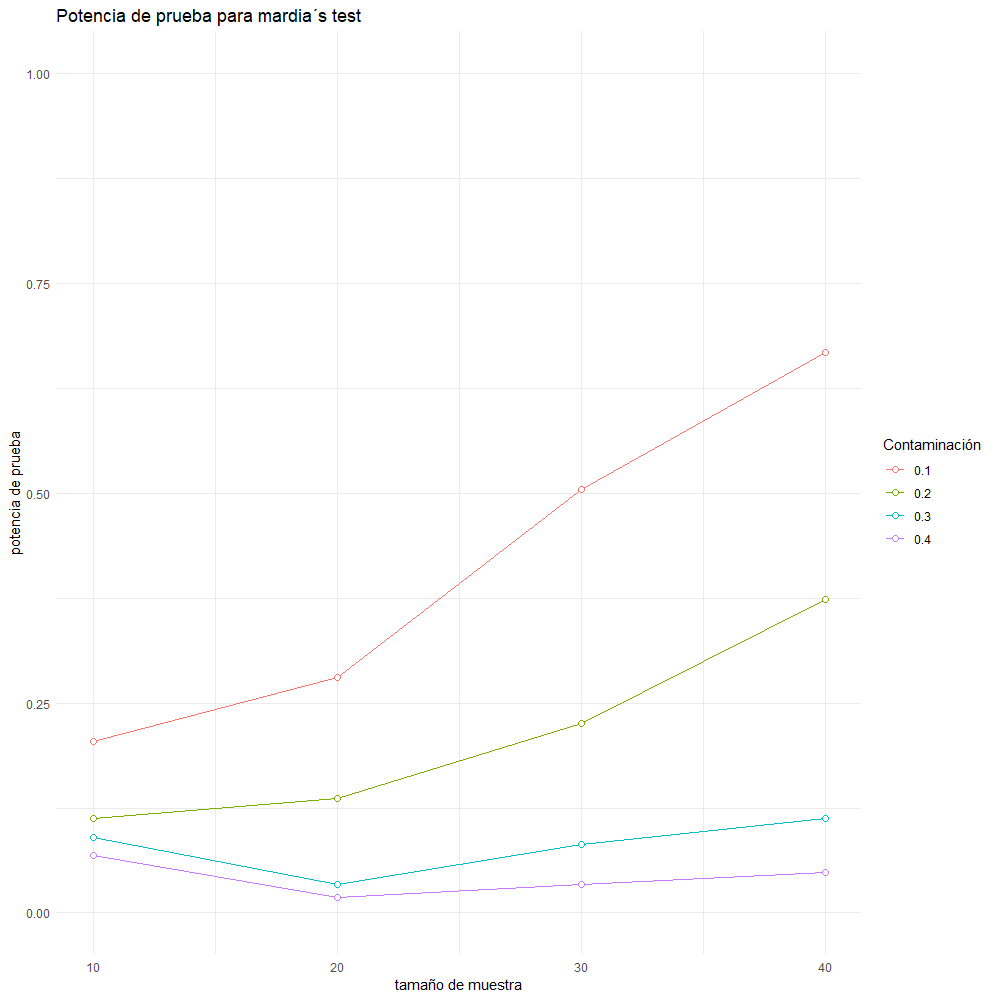
\includegraphics[width=\linewidth]{grafica de prueba.png}
\caption{grafica de prueba.}
\label{fig:foo}
\end{figure}

\newpage

\hypertarget{references}{%
\section{References}\label{references}}

{[}1{]} Allison, PD. (1995). Survival Analysis Using the SAS System: A
practical guide, Cary, NC:SAS Institute Inc., 292 pp.

{[}2{]} COX, D. R. Regression Models and Life Tables (with Discussion),
Journal of The Royal Statistical Society, Series B, 34, 187-220, 1972.

{[}3{]} ALLISON, P.D. Discrete-Time Methods for the Analysis of Event
Histories, In Sociological Methodology 1982, ed.~S. Leinhardt, San
Francisco, CA: Jossey-Bass, 1982.

\end{document}
